{%
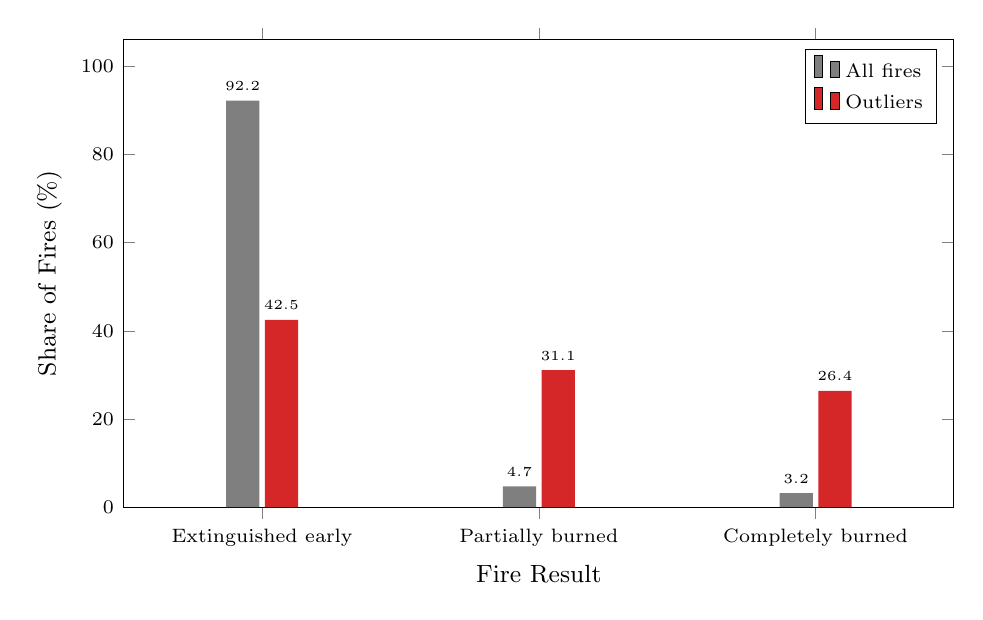
\begin{tikzpicture}
\begin{axis}[
  width=\columnwidth, height=0.62\columnwidth,
  ybar, bar width=12pt, ymin=0, ymax=106,
  symbolic x coords={Extinguished early,Partially burned,Completely burned}, xtick=data,
  enlarge x limits=0.25,
  xlabel={Fire Result}, ylabel={Share of Fires (\%)},
  tick label style={font=\scriptsize}, label style={font=\small},
  nodes near coords={\pgfmathprintnumber[fixed,fixed zerofill,precision=1]{\pgfplotspointmeta}},
  every node near coord/.append style={font=\tiny},
  legend style={at={(0.98,0.98)}, anchor=north east, font=\scriptsize},
  legend cell align=left,
]
\addplot[fill={rgb,255:red,127;green,127;blue,127}, draw=none] coordinates {(Extinguished early,92.2) (Partially burned,4.7) (Completely burned,3.2)};
\addlegendentry{All fires}
\addplot[fill={rgb,255:red,214;green,39;blue,40}, draw=none] coordinates {(Extinguished early,42.5) (Partially burned,31.1) (Completely burned,26.4)};
\addlegendentry{Outliers}
\end{axis}
\end{tikzpicture}%
}